\documentclass{article}

\usepackage[left=2cm,right=2cm,top=2cm,bottom=2cm]{geometry} 

\usepackage[utf8]{inputenc}   % otra alternativa para los caracteres acentuados y la "ñ"
\usepackage[           spanish % para poder usar el español
                      ,es-tabla % para los captions de las tablas
                       ]{babel}   
\decimalpoint %para usar el punto decimal en vez de coma para los números con decimales

%\usepackage{beton}
%\usepackage[T1]{fontenc}

\usepackage{parskip}
\usepackage{xcolor}

\usepackage{caption}

\usepackage{enumerate} % paquete para poder personalizar fácilmente la apariencia de las listas enumerativas

\usepackage{graphicx} % figuras
\usepackage{subfigure} % subfiguras

\usepackage{amsfonts}
\usepackage{amsmath}

\usepackage{colortbl}

\usepackage{listings}
\lstset
{ %Formatting for code in appendix
    language=python,
    basicstyle=\footnotesize,
    stepnumber=1,
    showstringspaces=false,
    tabsize=1,
    breaklines=true,
    breakatwhitespace=false,
}

\definecolor{softpink}{rgb}{1,0.8,1}
	
\usepackage{float} % para controlar la situación de los entornos flotantes

\restylefloat{figure}
\restylefloat{table} 
\setlength{\parindent}{0mm}


\usepackage[bookmarks=true,
            bookmarksnumbered=false, % true means bookmarks in 
                                     % left window are numbered
            bookmarksopen=false,     % true means only level 1
                                     % are displayed.
            colorlinks=true,
            allcolors=blue,
            urlcolor=blue]{hyperref}
\definecolor{webblue}{rgb}{0, 0, 0.5}  % less intense blue

\renewcommand{\thesection}{\arabic{section}}

\title{\Huge Desarrollo de Aplicaciones para Internet \\ Práctica 10 \vspace{10mm}}

\author{\huge David Cabezas Berrido \vspace{10mm} \\ 
  \huge Grupo del Martes \vspace{10mm} \\ \huge dxabezas@correo.ugr.es \vspace{10mm}}

\begin{document}
\maketitle
\pagebreak
\tableofcontents
\pagebreak

\section{Resumen de la aplicación}
Comenzamos proporcionando una breve descripción de la funcionalidad de la aplicación.

Al entrar en \texttt{0.0.0.0:5000} somos redirigidos a \texttt{/home},
donde recibimos un mensaje de bienvenida. A la izquierda de la barra
de navegación tenemos un enlace a \texttt{/home} con el nombre de
Práctica 10 (que también se utiliza como título de la pestaña) y el
logo de Capsule-Corp (que también se utiliza como favicon), a la
derecha de este enlace, tenemos otro con el nombre de Pokemon que nos
lleva a \texttt{/pokemon}, donde podemos visualizar, consultar y
editar la base de datos de Pokemon gestionada con \textit{MongoDB}. El siguiente
enlace de la barra de navegación tiene el nombre Estadísticas y abre
un menú desplegable con enlaces a dos páginas donde visualizamos
gráficos con estadísticas sobre los Pokemon de la base de datos.

En la parte derecha de la barra de navegación tenemos un campo con la
fecha y hora actual, que se actualiza cada segundo, y un botón para
cambiar la apariencia de la página entre modo clásico y modo nocturno.

Por último, tenemos un footer con el nombre del autor.

\begin{figure}[H]
  \centering
  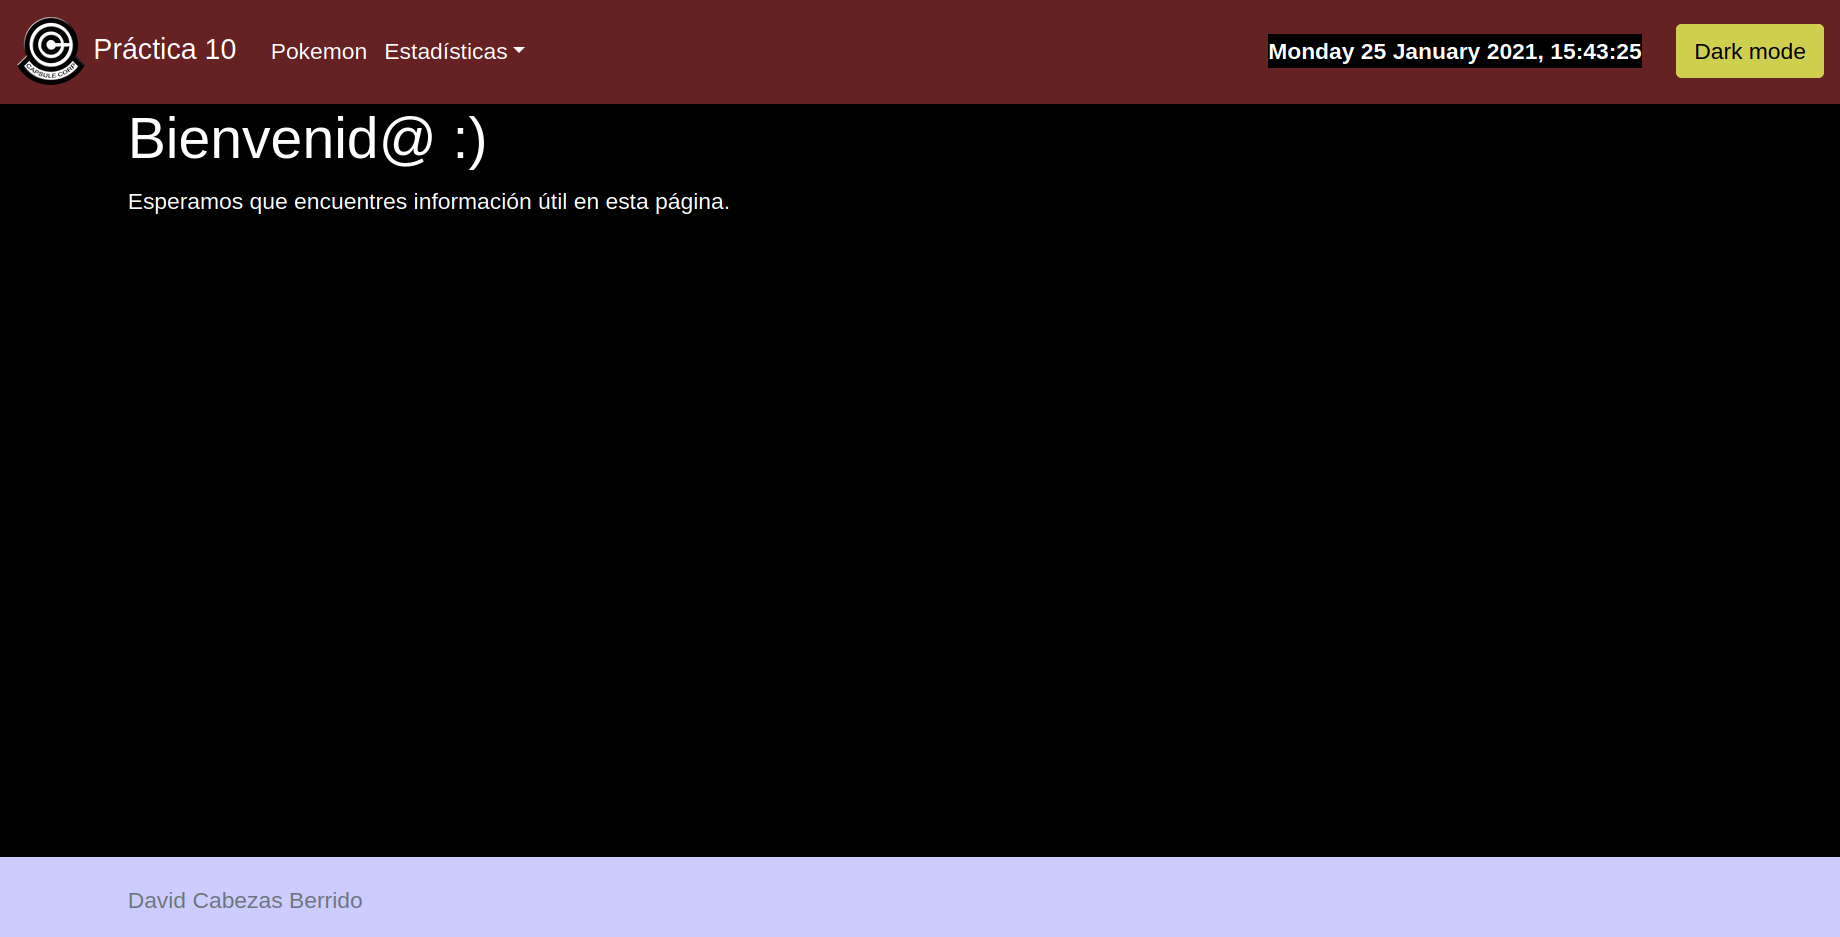
\includegraphics[width=180mm]{imgs/home}
  \caption{Página de bienvenida.}
  \label{fig:home}
\end{figure}

En la página \texttt{/pokemom}, tenemos formularios para buscar en la
base de datos de Pokemon por número (se mostrará el Pokemon
correspondiente a dicho número, en caso de que exista), por nombre (se
mostrarán los Pokemon cuyo nombre contenga la cadena introducida, sin
diferenciar mayúsculas y minúsculas) y por tipo (análogo a nombre,
pero la cadena estará contenida en alguno de los tipos de los
Pokemon). También hay un formulario para buscar por nombre y tipo a la
vez, realizando la intersección de las búsquedas por nombre y por tipo
antes descritas. A la derecha, hay un botón que permite añadir un
nuevo Pokemon a la base de datos, introuciendo sus datos en un
formulario que se proporciona al pulsar el botón.

Debajo, se listan los Pokemon que satisfacen los criterios de
búsqueda, cada uno con varios datos y un botón para editar o borrar el
Pokemon.

\begin{figure}[H]
  \centering
  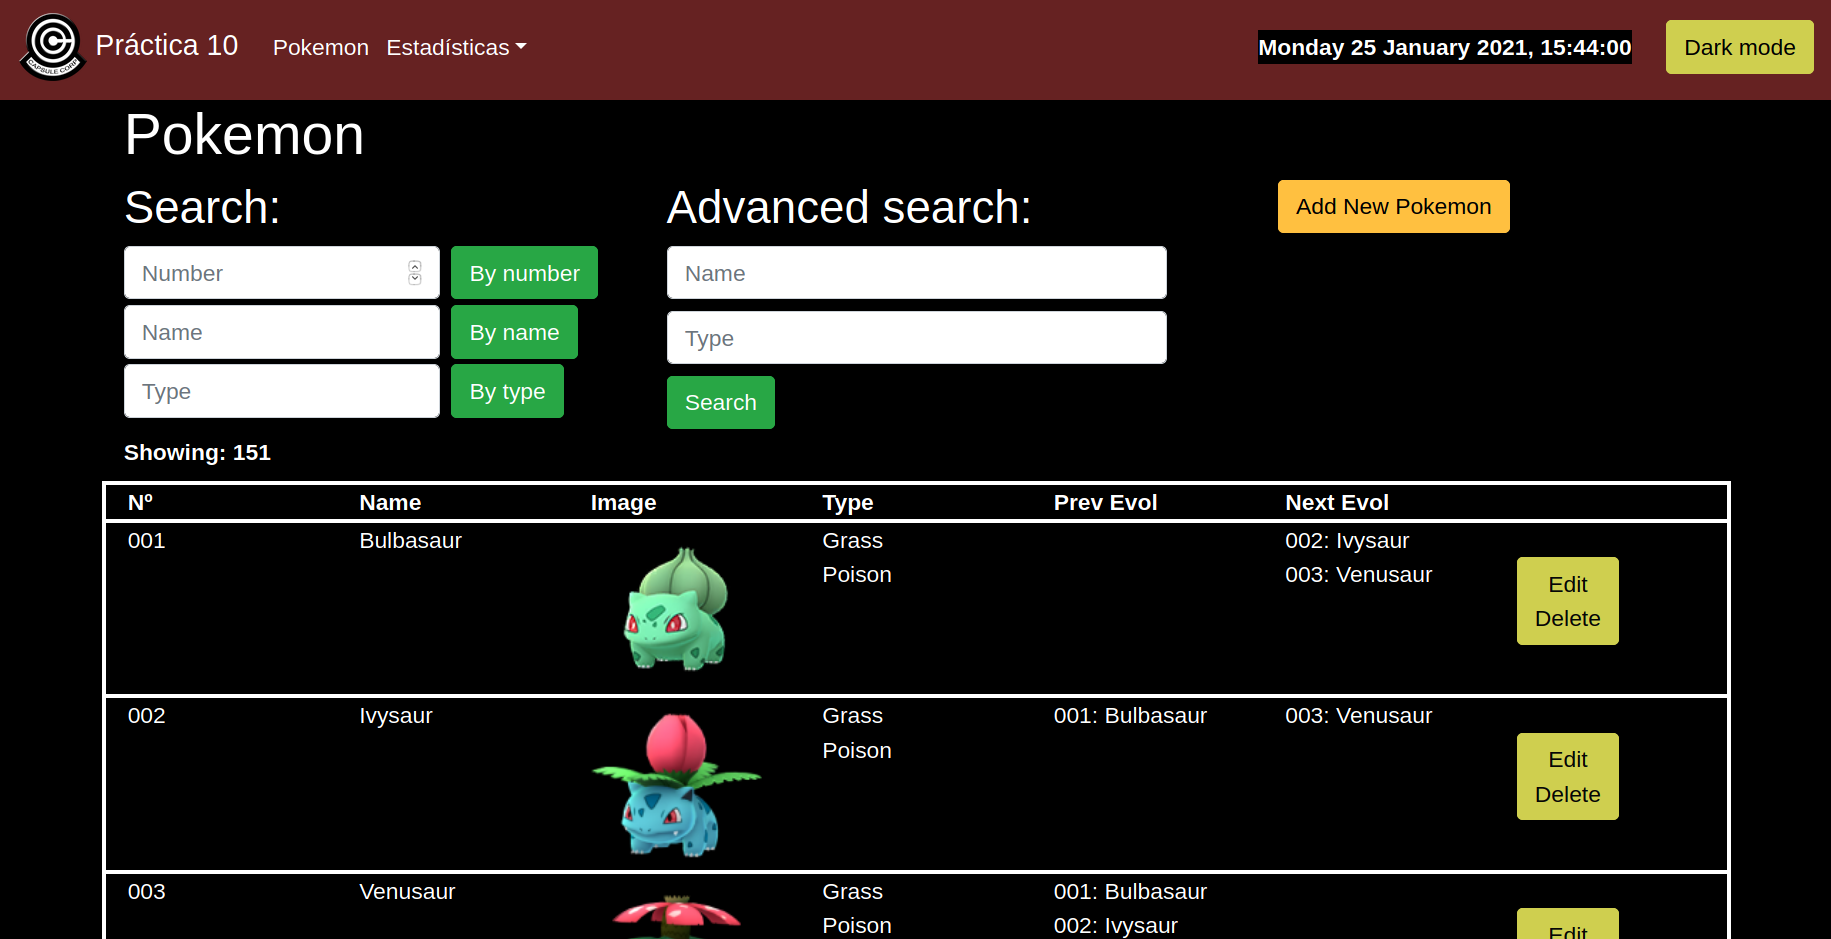
\includegraphics[width=180mm]{imgs/pokemon}
  \caption{Base de datos de Pokemon.}
  \label{fig:pokemon}
\end{figure}

\section{Funcionalidad front-end}
Detallamos cada una de las funcionalidades que hemos implementado con
Javascript en el front-end, puesto que es el principal objetivo de la
práctica.

\subsection{Modo nocturno}

Esta funcionalidad ya fue implementada en la Práctica 8, pero la
resaltamos porque hemos conseguido resolver un inconveniente que
presentaba.

Implementamos esta funcionalidad en el fichero \texttt{dark-mode.js}
de la carpeta \texttt{static}. Tenemos una variable llamada
\texttt{mode} que utilizamos a modo de flag, tomando los valores
\texttt{classic} (inicialmente) y \texttt{dark}, almacenamos esta
variable en \texttt{localStorage}. La función \texttt{change\_mode} se
encarga de alternar el valor de esta variable, almacenarlo en el
almacenamiento local y llamar a \texttt{set\_mode}, que lee el valor
de \texttt{mode} de \texttt{localStorage} y cambia el estilo de la
página añadiendo o eliminando la clase \texttt{dark-mode} a la lista
de clases del cuerpo de la página web. En el archivo
\texttt{static/style.css} nos encargamos de poner el texto de los
objetos con esta clase con fondo negro y texto blanco.  El script se
encarga también de llamar a \texttt{set\_mode} cada vez que se carga
la página para evitar que se restablezca el modo clásico al cambiar de
ruta dentro de la página.

El botón para cambiar de modo, simplemente llama a la función
\texttt{change\_mode} en cada click.

En la Práctica 8, este código estaba en el mismo script que el resto
del código JavaScript, que se cargaba al final del HTML, por lo que al
cambiar de dirección mientras se estaba en modo nocturno, se
visualizaba un ``flash'' blanco y volvía a fondo negro. Esto se debía
a que la página cargaba en su configuración por defecto y
posteriormente se ejecutaba el script que fijaba el modo
nocturno. Para solucionar este problema, cargamos el script al
principio de la etiqueta \texttt{body}, de tal forma que el cuerpo de
la página cargue directamente con el estilo correspondiente.

\subsection{Fecha y hora}

Añadimos un campo en la barra de navegación que indica la fecha y hora
actual. Para ello, añadimos un elemento al HTML con el id
\texttt{date} e implementamos en el fichero \texttt{static/date.js} la
función \texttt{printTime}. Esta función crea un objeto \texttt{Date}
(que por defecto se inicializa con la fecha y hora actual), lo
formatea como un string de la forma que queremos (utilizamos dos
listas constantes para obtener el día de la semana y el mes como
string, y fijamos las horas, minutos y segundos a dos dígitos enteros)
y modifica el \texttt{innerHTML} del elemento con id \texttt{date}
para que la muestre.

Con la función \texttt{setInterval}, podemos llamar a
\texttt{printTime} cada segundo para que se actualice la hora.

Esta forma de implementar un campo con fecha y hora la he conseguido
modificando un ejemplo que encontré en el
\href{https://www.sololearn.com/learning/1024}{curso de JavaScript de
  \textit{SoloLearn}}.

\subsection{Gráficos y estadísticas}

Utilizando la librería
\href{https://www.highcharts.com/}{\textit{Highcharts}} para mostrar
en forma de gráficos algunas estadísticas de la base de datos de
Pokemon. Otra alternativa para esta tarea sería la librería
\href{https://d3js.org/}{\textit{3D.js}}, pero tras observar algunas
demos en sus respectivas páginas, nos decantamos por
\textit{Highcharts}, ya que los códigos para generar gráficos con esta
librería son más cortos y me parecen más intuitivos. Además, los
gráficos de \textit{Highcharts} son interactivos, mientras que los
ejemplos que he visto de gráficos con \textit{3D.js} generaban simples
imágenes.

  El primer gráfico que generamos es un gráfico de barras que
  representa el \textbf{número de Pokemon de cada tipo} en la base de
  datos. En primer lugar, buscamos los diferentes tipos en la base de
  datos con la función \texttt{distinct} de Mongo:
\begin{verbatim}
types=db.samples_pokemon.distinct("type") # Lista de tipos
\end{verbatim}
  A continuación, combinamos \texttt{count} con una sencilla consulta
  para obtener el número de Pokemon en la base de datos que tienen
  cada tipo. Hay que tener en cuenta que un Pokemon puede tener uno o dos tipos.
\begin{verbatim}
for t in types:
    data[t]=db.samples_pokemon.find({"type":t}).count() # Número de Pokemon de cada tipo
\end{verbatim}
  Finalmente, renderizamos el template \texttt{stats-type} y pasamos
  como parámetros la lista de tipos y una lista con el número de
  Pokemon de cada tipo. Modificamos el código de
  \href{https://www.highcharts.com/docs/getting-started/your-first-chart}{este
    ejemplo} para generar el siguiente gráfico de barras:

\begin{figure}[H]
  \centering
  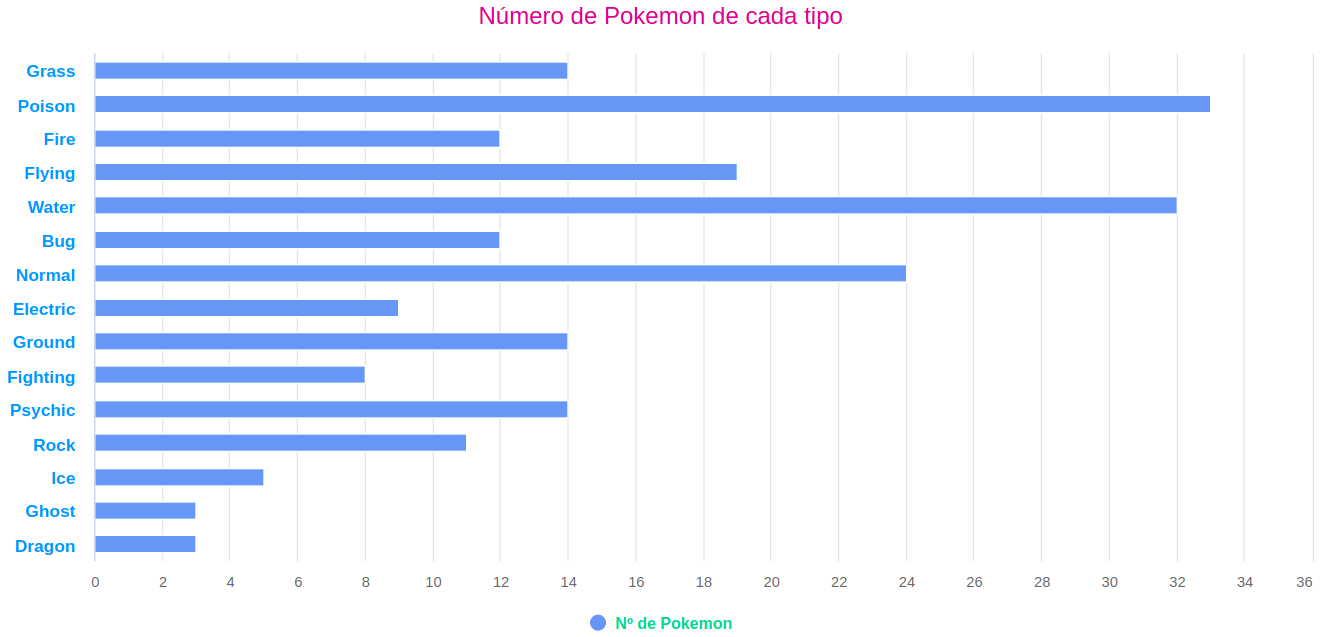
\includegraphics[width=190mm]{imgs/stats-type}
  \caption{Gráfico con el número de Pokemon de cada tipo.}
  \label{fig:stats-type}
\end{figure}

Aquí hemos tenido que resolver un importante problema: el carácter
\texttt{'} se renderiza en HTML como \texttt{\&\#39;}. Al utilizar una
lista de strings en \textit{Flask} como entrada para \texttt{categories} (la
lista de tipos), observamos (con inspaccionar elemento) que
\begin{verbatim}
categories: {{types}}
\end{verbatim}
se renderiza como
\begin{verbatim}
categories: [&#39;Grass&#39;, &#39;Poison&#39;, &#39;Fire&#39;, &#39;Flying&#39;,...
\end{verbatim}
y recibimos el error:
\begin{verbatim}
Uncaught SyntaxError: expected expression, got '&'
\end{verbatim}
Para solucionar este problema, añadimos el filtro \texttt{safe} de esta forma: 
\begin{verbatim}
categories: {{types|safe}}
\end{verbatim}
como sugiere \href{https://stackoverflow.com/questions/20026975/using-a-flask-variable-as-data-source-for-highcharts}{esta página}.

El segundo gráfico que generamos es un gráfico de tarta que representa
el \textbf{número de Pokemon en cada etapa de evolución}, separa los
Pokemon en tres categorías, según si han evolucionado ninguna, una o
dos veces (algunos Pokemon tienen tres fases de evolución, otros dos y
otros sólo una, por lo que no evolucionan). Primero, obtenemos el
número de Pokemon en cada una de estas tres categorías, consultando la
longitud de la lista en el campo \texttt{prev\_evolution},
\begin{verbatim}
# Han evolucionado una vez
count[1]=db.samples_pokemon.find({"prev_evolution":{ "$exists": True, "$size": 1}}).count()
# Han evolucionado dos veces
count[2]=db.samples_pokemon.find({"prev_evolution":{ "$exists": True, "$size": 2}}).count()
# No han evolucionado nunca: lista de longitud 0 o no definida
count[0]=db.samples_pokemon.find({"prev_evolution":{ "$exists": False}}).count()
count[0]+=db.samples_pokemon.find({"prev_evolution":{ "$exists": True, "$size": 0}}).count()
\end{verbatim}

Renderizamos ahora el template \texttt{stats-evol} con estos recuentos
como parámetro, donde modificamos el código de \href{}{este ejemplo}
para generar el siguiente gráfico de tarta:

\begin{figure}[H]
  \centering
  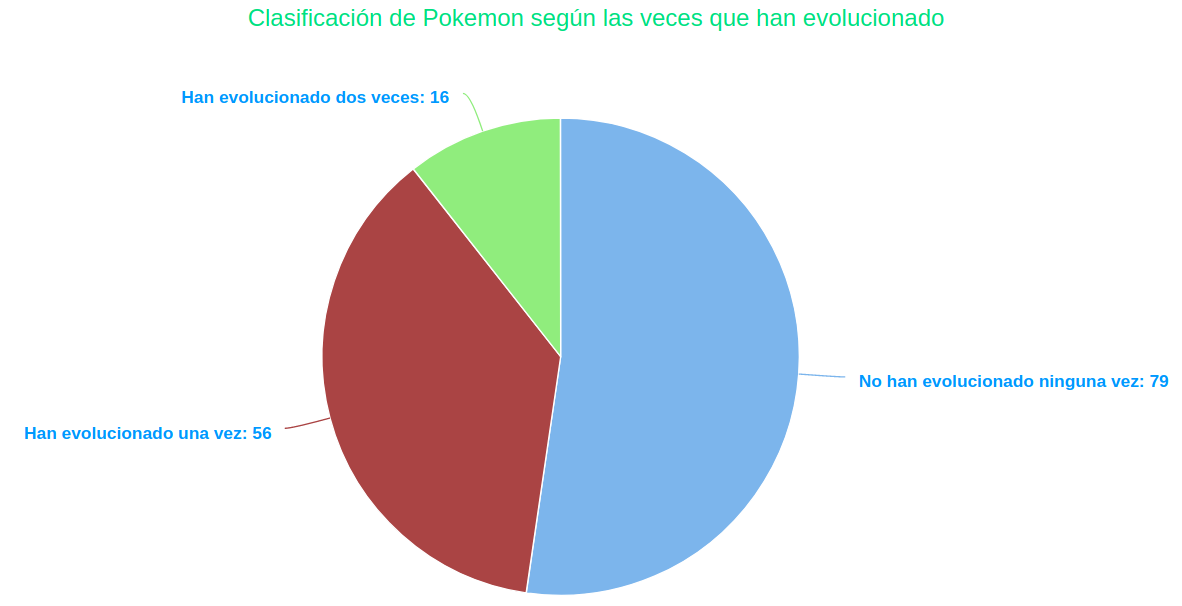
\includegraphics[width=190mm]{imgs/stats-evol}
  \caption{Gráfico con el número de Pokemon en cada etapa de evolución.}
  \label{fig:stats-evol}
\end{figure}

Sería apetecible que el estilo de los gráficos se adaptara al de la
página (clásico y nocturno), esto presenta varias dificultades. En
\href{https://www.highcharts.com/forum/viewtopic.php?t=44170}{este
  post} del foro de \textit{Highcharts}, se sugiere que no es posible
cambiar las opciones de \textit{Highcharts} de forma dinámica y ofrece
dos alternativas: una es destruir y volver a crear el gráfico, y la
otra es utilizar \texttt{update} para modificar el estilo del
gráfico. Se puede elegir un estilo fácilmente en el momento de generar
el gráfico leyendo la variable \texttt{mode} de \texttt{localStorage},
pero a la hora de cambiar de modo con un gráfico en pantalla, habría
que actualizarlo, lo cual es bastante complejo. Al no encontrar
ninguna solución satisfactoria, decidimos darle a los gráficos fondo
transparante y colores que contrasten bien con ambos fondos (blanco y
negro). Para modificar los colores, estilos y fuentes de los gráficos
nos basamos en
\href{https://stackoverflow.com/questions/8607365/how-to-change-the-text-color-in-highcharts}{este
  ejemplo}.

\section{Mapas}


  
\end{document}
